\documentclass[tikz, border=2pt]{standalone}

\usepackage{amsmath,amssymb}
\usepackage{pgfplots}
\pgfplotsset{compat=1.18}
\usepackage{xcolor}

\definecolor{utnblue}{RGB}{0, 51, 102}

\begin{document}
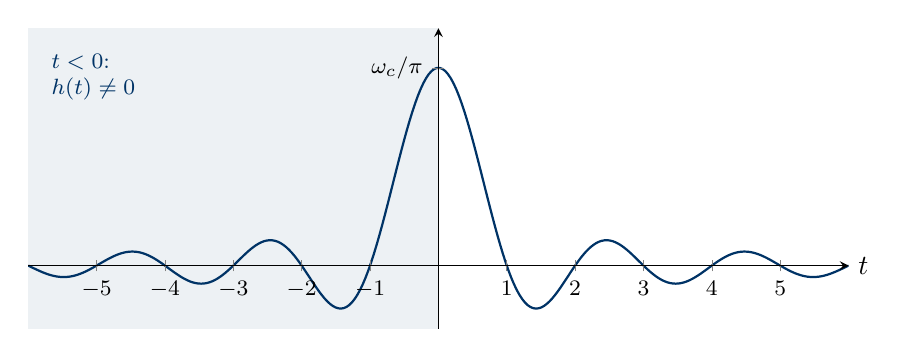
\begin{tikzpicture}
\begin{axis}[
    width=12cm, height=5.4cm,
    axis lines=middle,
    axis on top=true,
    enlargelimits=false,
    tick label style={font=\footnotesize},
    label style={font=\small},
    xlabel={$t$},
    every axis x label/.style={at={(ticklabel* cs:1)}, anchor=west},
    xmin=-6, xmax=6, ymin=-0.32, ymax=1.2,
    xtick={-5,-4,-3,-2,-1,1,2,3,4,5},
    ytick={1}, yticklabels={$\omega_c/\pi$},
    clip mode=individual,
]
% region t<0 (no causal)
\fill[utnblue!7] (axis cs:-6,-0.32) rectangle (axis cs:0,1.2);
\node[font=\footnotesize, utnblue, anchor=north west, align=left]
    at (axis cs:-5.8,1.12) {$t<0$:\\ $h(t)\neq 0$};
% h(t) = sinc(pi t) normalizado (wc = pi)
\addplot[utnblue, thick, samples=300, domain=-6:6] {sin(deg(pi*x))/(pi*x)};
\end{axis}
\end{tikzpicture}
\end{document}
